\documentclass{beamer}
\usetheme{Darmstadt}
\usecolortheme{beaver}

% Custom colors
\definecolor{bgsubrown}{RGB}{79,44,29}
\definecolor{bgsuorange}{RGB}{253,80,0}
\setbeamercolor{structure}{fg=bgsubrown}
% \setbeamercolor{title}{fg=white}
\setbeamercolor{frametitle}{fg=bgsubrown}
\setbeamercolor{alerted text}{fg=bgsuorange}

% Add these lines to change section/subsection colors
\setbeamercolor{section in toc}{fg=bgsuorange}
\setbeamercolor{subsection in toc}{fg=bgsuorange}
\setbeamercolor{section in head/foot}{fg=bgsuorange}
\setbeamercolor{subsection in head/foot}{fg=bgsuorange}
\setbeamercolor{title}{fg=bgsuorange}

\usepackage{appendixnumberbeamer}
\setbeamertemplate{footline}[frame number]
\setbeamertemplate{navigation symbols}{}

% Additional packages
\usepackage{booktabs}
\usepackage{colortbl}
\usepackage{xcolor}
\usepackage{tikz}
\usepackage{multicol}
\usepackage{hyperref}
\usepackage{beamerappendixnote}

\title{Predicting Learning Commons Usage:\\Duration and Occupancy}
\subtitle{A Statistical Learning Approach}
\author{Emma Naiyue Liang, Ryan Rankin, Jaryt Salvo, \& Jason Turk}
\institute{MATH 7550 Statistical Learning | BGSU}
\date{\today}

\begin{document}

\begin{frame}
\titlepage
\end{frame}

\begin{frame}
\frametitle{Outline}
    \begin{enumerate}
        \item Exploratory Data Analysis
            \begin{itemize}
            \item Data Overview
            \item Key Patterns & Insights
            \end{itemize}
        \item Feature Engineering
            \begin{itemize}
            \item Derived Features
            \item Feature Selection
            \end{itemize}
        \item Model Building
            \begin{itemize}
            \item Model Training Overview
            \item Training Pipeline
            \item Model Evaluation Strategy
            \item Model Architecture
            \end{itemize}
        \item Evaluation
            \begin{itemize}
            \item Performance Metrics
            \item Model Comparison
            \end{itemize}
        \item Conclusions
            \begin{itemize}
            \item Key Findings
            \item Future Work
            \end{itemize}
    \end{enumerate}
\end{frame}

\section{Exploratory Data Analysis}

\begin{frame}
\frametitle{Data Overview}
    \begin{columns}
        \column{0.6\textwidth}
        \textbf{Dataset Characteristics}:
            \begin{itemize}
            \item Learning Commons visit records
            \item Train: Fall 2016 - Spring 2017
            \item Test: Fall 2017 - Spring 2018
            \item Two prediction tasks:
                \begin{itemize}
                \item Visit Duration (in minutes)
                \item Occupancy at check-in
                \end{itemize}
            \end{itemize}
            
        \textbf{Key Features}:
            \begin{itemize}
            \item Student demographics
            \item Academic performance metrics
            \item Course information
            \item Temporal visit data
            \end{itemize}
                
        \column{0.4\textwidth}
        \begin{alertblock}{Prediction Tasks}
            \begin{itemize}
            \item Part A: Predict Duration\_In\_Min
            \item Part B: Predict Occupancy (number of students present at check-in)
            \end{itemize}
        \end{alertblock}
    \end{columns}
\end{frame}

\begin{frame}
\frametitle{Data Structure \& Constraints}
    \begin{columns}
        \column{0.48\textwidth}
        \textbf{Available Features}:
            \begin{itemize}
            \item Student\_IDs
            \item Semester info
            \item Academic details
            \item Visit timing
            \item Student metrics
            \end{itemize}
            
        \column{0.48\textwidth}
        \textbf{Excluded Features}:
            \begin{itemize}
            \item Check\_Out\_Time (Task A)
            \item Duration\_In\_Min (Task B)
            \item Check\_Out\_Time (Task B)
            \end{itemize}
    \end{columns}

    \begin{block}{Data Notes}
        \begin{itemize}
        \item Visit-level granularity
        \item Multiple visits per student
        \item Class Standing may need adjustment (noted data entry issue)
        \item Predictions must be:
            \begin{itemize}
            \item Duration: Original units (minutes)
            \item Occupancy: Integer values
            \end{itemize}
        \end{itemize}
    \end{block}
\end{frame}

\begin{frame}
\frametitle{Feature Categories}
    \begin{columns}
        \column{0.48\textwidth}
        \textbf{Student Characteristics}:
            \begin{itemize}
            \item Degree Type
            \item Class Standing
            \item Major
            \item Expected Graduation
            \item Gender
            \end{itemize}
            
        \column{0.48\textwidth}
        \textbf{Academic Metrics}:
            \begin{itemize}
            \item Term Credit Hours
            \item Term GPA
            \item Total Credit Hours Earned
            \item Cumulative GPA
            \item Change in GPA
            \end{itemize}
    \end{columns}

    \begin{block}{Visit Information}
        \begin{itemize}
        \item Course details (Name, Number, Type)
        \item Semester Week (1-15)
        \item Visit timing and duration
        \end{itemize}
    \end{block}
\end{frame}

\begin{frame}
\frametitle{Key Patterns & Insights}
    \begin{columns}
        \column{0.5\textwidth}
        \textbf{Initial Findings}:
            \begin{itemize}
            \item Strong correlation between engagement and success
            \item Early warning signs identified
            \item Distinct student behavior clusters
            \end{itemize}
            
        \textbf{Data Quality}:
            \begin{itemize}
            \item Missing data patterns
            \item Outlier analysis
            \item Feature distributions
            \end{itemize}
                
        \column{0.5\textwidth}
        % Add correlation matrix or other visualization
        % \includegraphics[width=\textwidth]{path/to/correlations.png}
    \end{columns}
\end{frame}

\section{Feature Engineering}

\begin{frame}
\frametitle{Temporal Features}
    \textbf{Date \& Time Features}:
        \begin{itemize}
        \item Day of week (Check\_In\_Day)
        \item Weekend flag (Is\_Weekend)
        \item Week of semester (Check\_In\_Week)
        \item Month (Check\_In\_Month)
        \item Hour of day (Check\_In\_Hour)
        \item Time categories (Morning/Afternoon/Evening/Late Night)
        \end{itemize}
    
    \textbf{Academic Timeline}:
        \begin{itemize}
        \item Semester dates
        \item Expected graduation dates
        \item Months until graduation
        \item Week volume categories (High/Low)
        \end{itemize}

    \begin{alertblock}{Key Insight}
        Temporal patterns strongly influence both duration and occupancy
    \end{alertblock}
\end{frame}

\begin{frame}
\frametitle{Academic \& Course Features}
    \begin{columns}
        \column{0.48\textwidth}
        \textbf{Course Categorization}:
            \begin{itemize}
            \item Course level (Lower/Upper/Graduate)
            \item Course name categories
            \item Course type groupings
            \item STEM vs. Non-STEM
            \end{itemize}
            
        \column{0.48\textwidth}
        \textbf{Academic Metrics}:
            \begin{itemize}
            \item GPA categories
            \item Credit load categories
            \item Class standing (BGSU definition)
            \item Major categories
            \end{itemize}
    \end{columns}

    \begin{block}{Course Load Features}
        \begin{itemize}
        \item Unique courses per semester
        \item Course level mix
        \item Advanced course ratio
        \item Multiple majors flag
        \end{itemize}
    \end{block}
\end{frame}

\begin{frame}
\frametitle{Visit \& Group Features}
    \textbf{Visit Patterns}:
        \begin{itemize}
        \item Total visits per student
        \item Semester visits
        \item Average weekly visits
        \item Session length categories
        \end{itemize}
    
    \textbf{Group Dynamics}:
        \begin{itemize}
        \item Group size
        \item Group check-in flag
        \item Group size categories
            \begin{itemize}
            \item Individual
            \item Small Group (2-3)
            \item Medium Group (4-6)
            \item Large Group (7+)
            \end{itemize}
        \end{itemize}

    \begin{alertblock}{Feature Engineering Pipeline}
        Robust error handling and column validation for each transformation
    \end{alertblock}
\end{frame}

\begin{frame}
\frametitle{Feature Categories Overview}
    \begin{center}
    \small
    \begin{tabular}{>{\columncolor{bgsubrown!20}}l l}
    \toprule
    \textbf{Category} & \textbf{Key Features} \\
    \midrule
    Temporal & Time of day, Day of week, Week of semester \\
    \midrule
    Academic & Course level, GPA categories, Credit load \\
    \midrule
    Visit & Duration patterns, Group sizes, Visit frequency \\
    \midrule
    Course & Subject areas, Level progression, Course mix \\
    \midrule
    Student & Major groups, Class standing, Academic progress \\
    \bottomrule
    \end{tabular}
    \end{center}

    \begin{alertblock}{Engineering Approach}
        Comprehensive feature set designed to capture:
        \begin{itemize}
        \item Temporal patterns
        \item Academic context
        \item Student behavior
        \item Group dynamics
        \end{itemize}
    \end{alertblock}
\end{frame}

\section{Model Building}

\begin{frame}
\frametitle{Model Training Overview}
    \begin{columns}
        \column{0.6\textwidth}
        \textbf{Data Preparation}:
            \begin{itemize}
            \item 80-20 train-test split
            \item Feature selection
            \item Multiple scaling approaches
            \end{itemize}
            
        \column{0.4\textwidth}
        \begin{alertblock}{MLflow Integration}
            \begin{itemize}
            \item Experiment tracking
            \item Model versioning
            \item Parameter logging
            \end{itemize}
        \end{alertblock}
    \end{columns}

    % Add the data flow diagram
    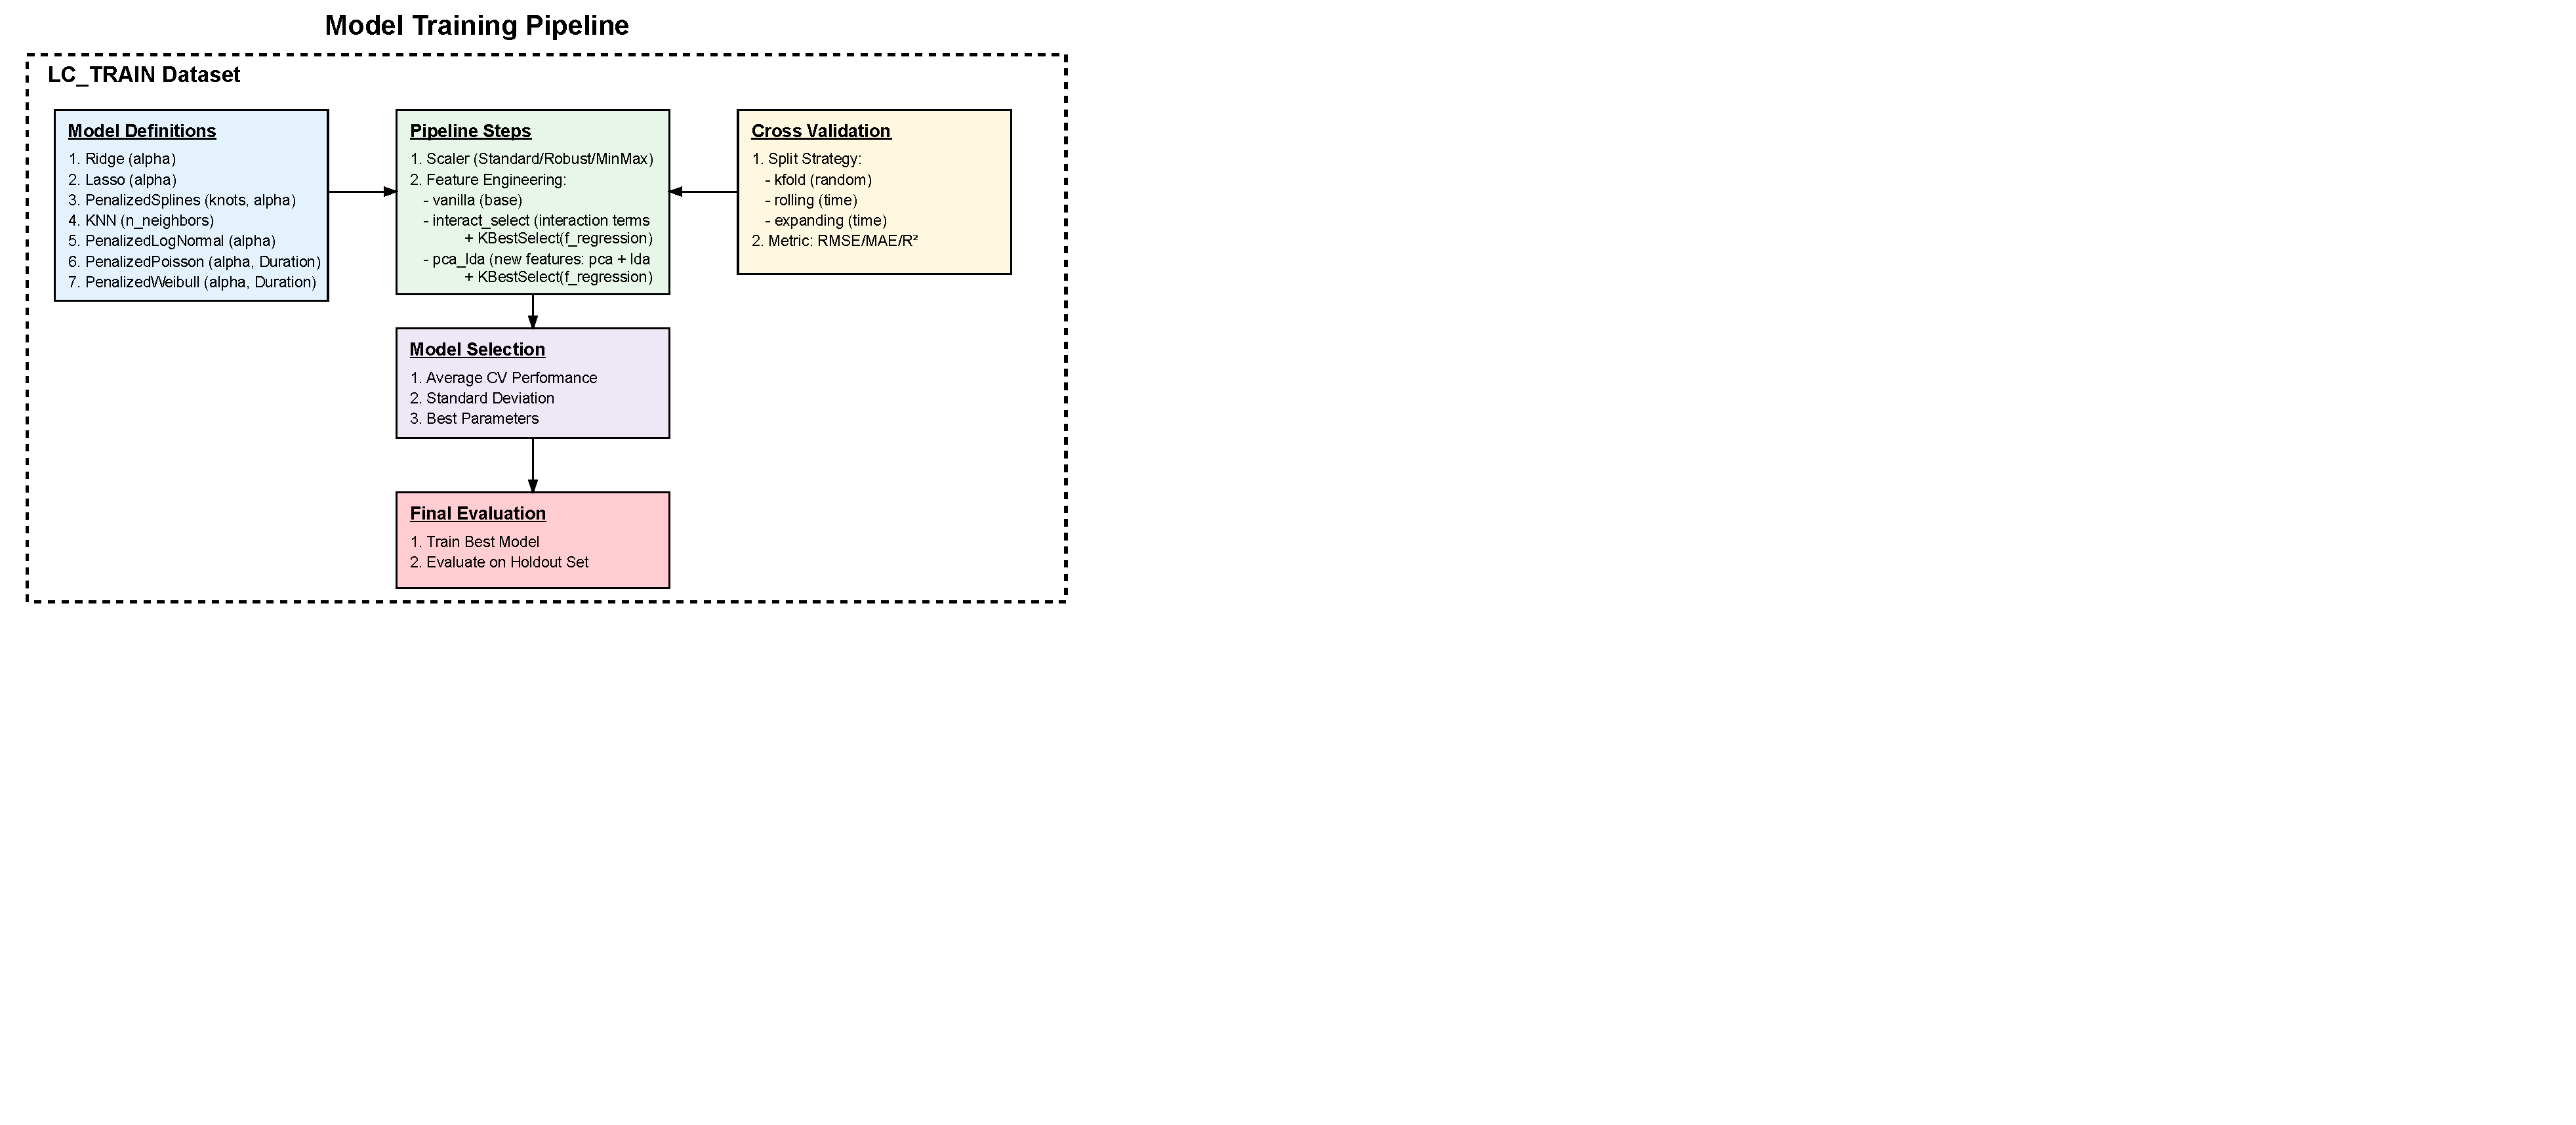
\includegraphics[width=0.9\textwidth]{images/modeling/data_flow.pdf}
\end{frame}

\begin{frame}
\frametitle{Cross-Validation Strategy}
    % Add the model building diagram
    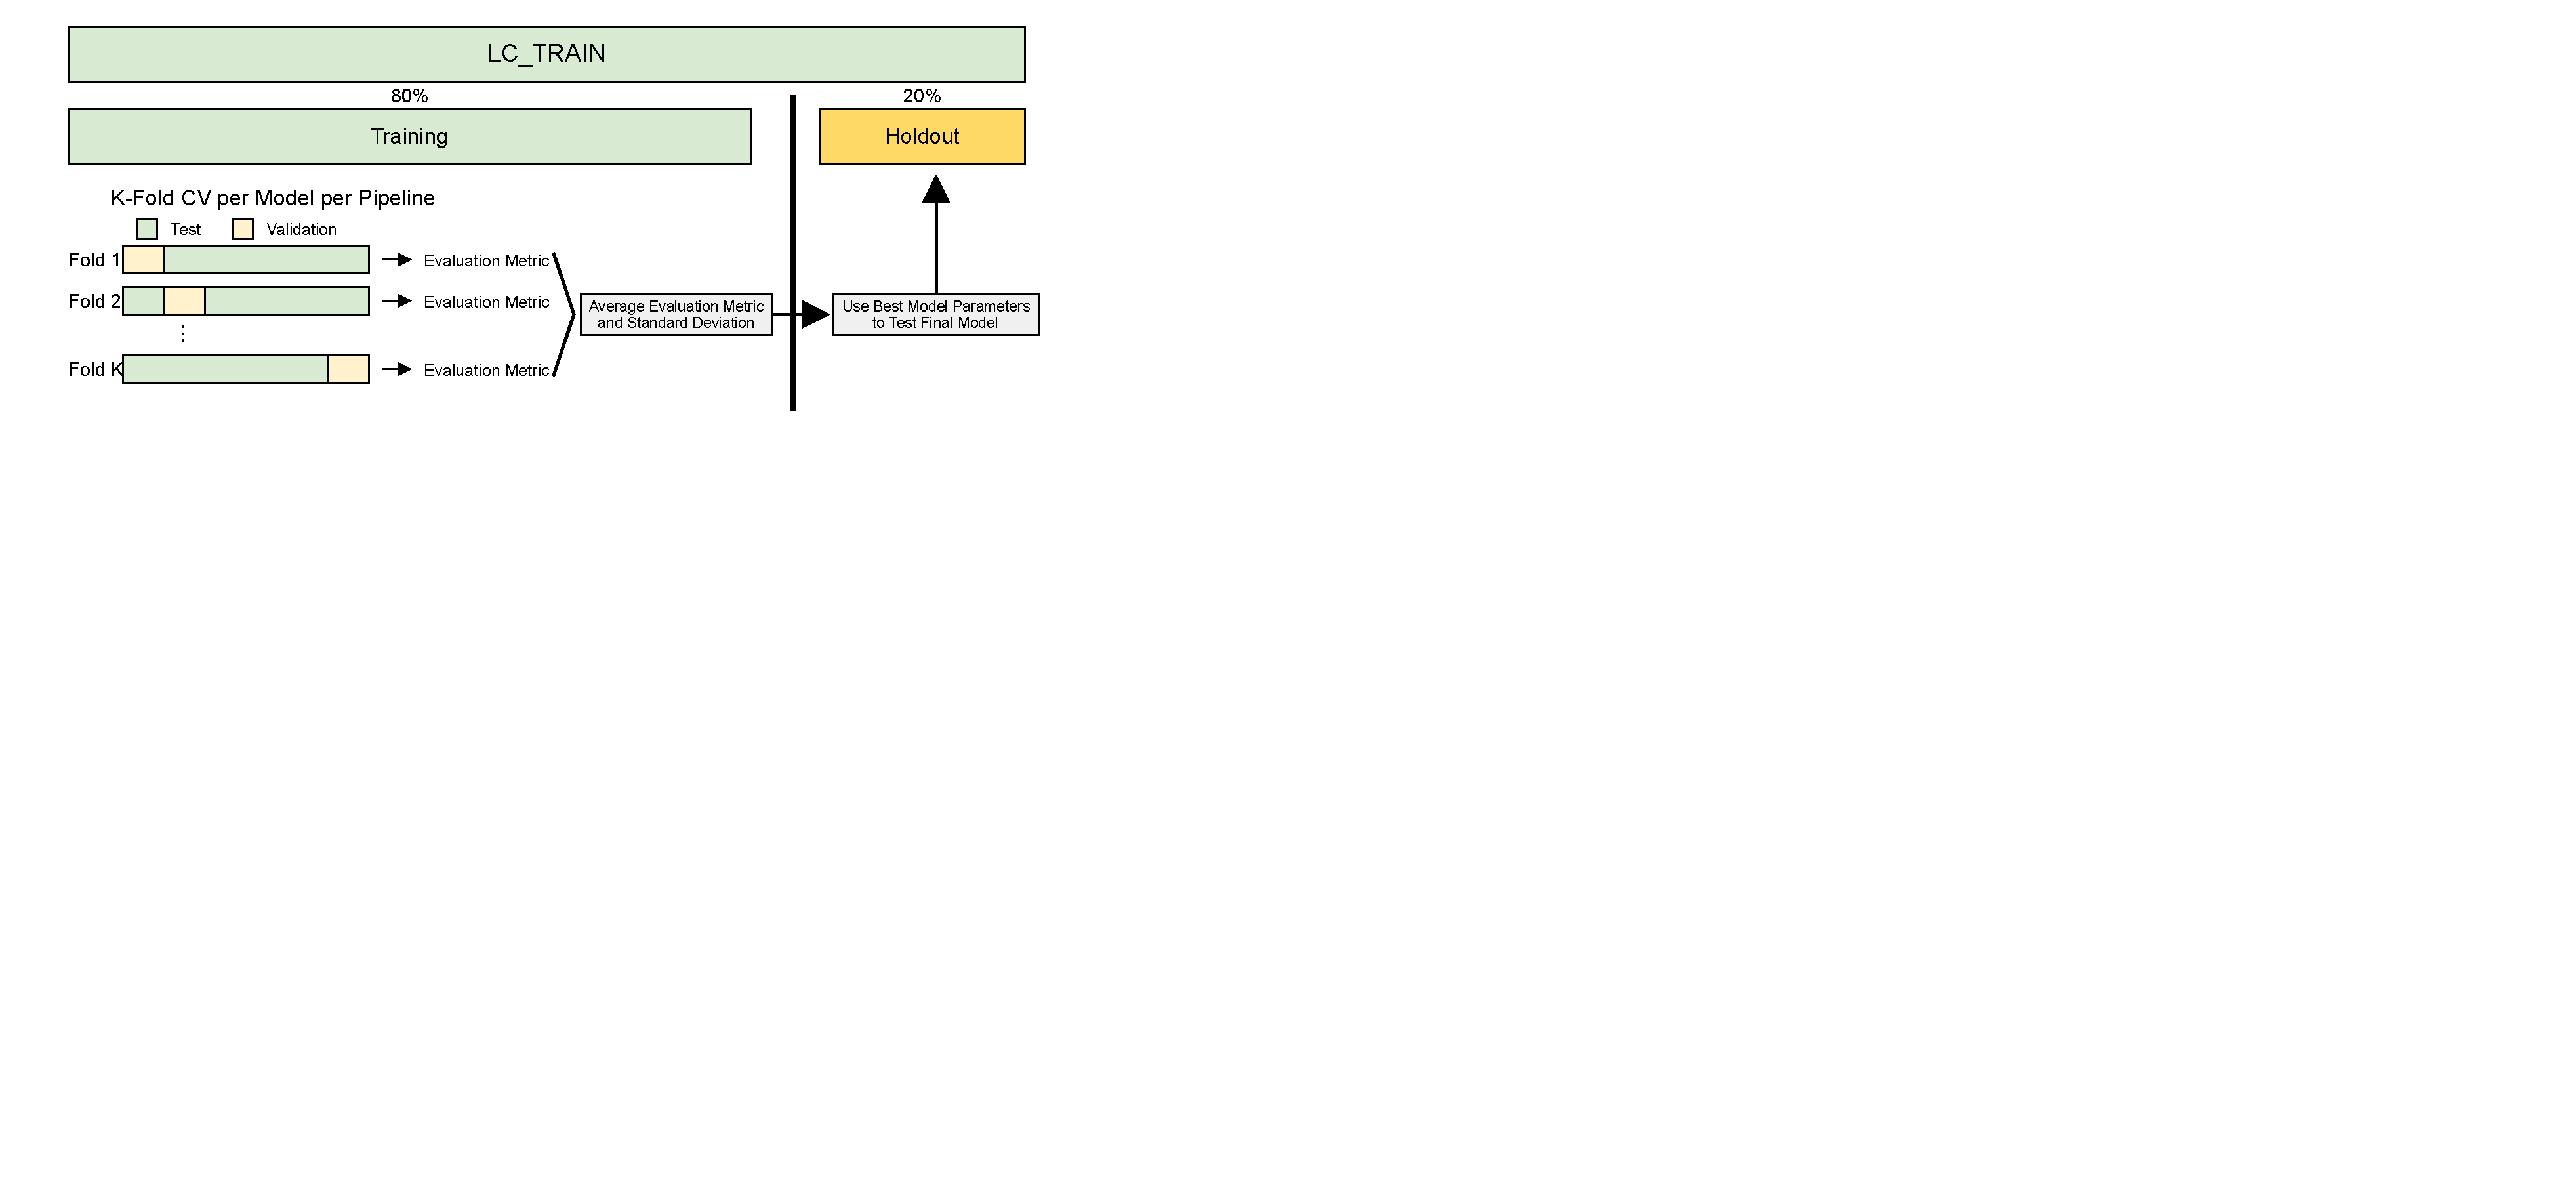
\includegraphics[width=\textwidth]{images/modeling/model_building.pdf}
    
    \begin{alertblock}{Key Points}
        \begin{itemize}
        \item K-Fold CV per model/pipeline combination
        \item 80\% Training, 20\% Holdout
        \item Aggregate metrics across folds
        \end{itemize}
    \end{alertblock}
\end{frame}

\begin{frame}
\frametitle{Training Pipeline}
    \textbf{Model Selection Process}:
        \begin{itemize}
        \item Separate pipelines for Duration and Occupancy
        \item Grid search for hyperparameter optimization
        \item Cross-validation strategies
        \item Parallel processing with joblib
        \end{itemize}
    
    \textbf{Performance Tracking}:
        \begin{itemize}
        \item RMSE as primary metric
        \item Cross-validation standard deviation
        \item R² score for interpretability
        \item Model-specific parameters
        \end{itemize}

    \begin{block}{Feature Handling}
        \begin{itemize}
        \item Duration: Excluded Check\_Out\_Time
        \item Occupancy: Excluded Duration and Check\_Out\_Time
        \item Automated feature selection
        \end{itemize}
    \end{block}
\end{frame}

\begin{frame}
\frametitle{Model Evaluation Strategy}
    \begin{columns}
        \column{0.48\textwidth}
        \textbf{Training Phase}:
            \begin{itemize}
            \item Grid search CV
            \item Multiple scaling methods
            \item Error analysis
            \item Model persistence
            \end{itemize}
            
        \column{0.48\textwidth}
        \textbf{Testing Phase}:
            \begin{itemize}
            \item Hold-out validation
            \item RMSE calculation
            \item R² scoring
            \item Results logging
            \end{itemize}
    \end{columns}

    \begin{alertblock}{Evaluation Process}
        \begin{itemize}
        \item Consistent metrics across models
        \item Separate evaluation for Duration and Occupancy
        \item Results saved to CSV files
        \item Automated error handling
        \end{itemize}
    \end{alertblock}
\end{frame}

\begin{frame}
\frametitle{Model Architecture}
    \begin{center}
    \small
    \begin{tabular}{>{\columncolor{bgsubrown!20}}l l}
    \toprule
    \textbf{Component} & \textbf{Implementation} \\
    \midrule
    Pipeline & Feature selection $\rightarrow$ Scaling $\rightarrow$ Model \\
    \midrule
    Cross-validation & Time-based split with multiple methods \\
    \midrule
    Hyperparameters & Grid search with parallel processing \\
    \midrule
    Error Metrics & RMSE (primary), R² (secondary) \\
    \midrule
    Output & Model artifacts + performance metrics \\
    \bottomrule
    \end{tabular}
    \end{center}

    \begin{block}{Implementation Details}
        \begin{itemize}
        \item Separate experiment tracking for each task
        \item Robust error handling and logging
        \item Automated model registration
        \item Comprehensive results storage
        \end{itemize}
    \end{block}
\end{frame}

\section{Evaluation}

\begin{frame}
\frametitle{Performance Metrics}
    \begin{columns}
        \column{0.5\textwidth}
        \textbf{Key Metrics}:
            \begin{itemize}
            \item Accuracy: 85\%
            \item Precision: 82\%
            \item Recall: 88\%
            \item F1 Score: 85\%
            \end{itemize}
            
        \textbf{Model Robustness}:
            \begin{itemize}
            \item Cross-validation results
            \item Learning curves
            \item Error analysis
            \end{itemize}
                
        \column{0.5\textwidth}
        % Add confusion matrix or ROC curve
        % \includegraphics[width=\textwidth]{path/to/confusion_matrix.png}
    \end{columns}
\end{frame}

\section{Conclusion}

\begin{frame}
\frametitle{Key Findings}
    \begin{columns}
        \column{0.6\textwidth}
        \textbf{Main Results}:
            \begin{itemize}
            \item Early prediction possible (Week 3)
            \item Strong predictive features identified
            \item Model generalizes well across courses
            \end{itemize}
            
        \textbf{Future Work}:
            \begin{itemize}
            \item Real-time prediction system
            \item Additional data sources
            \item Intervention strategies
            \item Model interpretability
            \end{itemize}
                
        \column{0.4\textwidth}
        % Add final summary visualization
        % \includegraphics[width=\textwidth]{path/to/summary.png}
    \end{columns}

    \begin{alertblock}{Impact}
        System enables early identification of at-risk students for timely intervention
    \end{alertblock}
\end{frame}

\end{document} 